As discussed in the previous section, an HPC software stack can be complex, and
the hardware features many of optimizations and offloads that can have
unpredictable effect on the performance on real-life applications. Because of
this, it is very challenging to predict the execution time of an application on
a given cluster, although it is an important problem to solve, in order to
improve applications' code, optimize libraries, and design more performant
hardware for the next generation. It is also important to be able to model the
behavior of hardware before making physical prototypes, because it accelerates
the development and reduces the costs of hardware design by orders of magnitude.
For software developers, testing on real-life clusters, or hardware that is not
available yet, can be difficult and costly (since clusters require a huge amount
of power, and often have many users which need to share the resources). This is
why simulators are a crucial tool for both hardware designers and software
developers in HPC.

\section{Tradeoff between performance and accuracy}

We can categorize simulators in a few groups, depending on their use case: for
hardware designers, most of the time simulators need to be a faithful emulator
of real-world hardware, to be able to fine tune the behavior of the circuit to
get the desired output. This type of simulation is called Cycle Accurate, Bit
Accurate (CABA) when modeling processing units (like CPUs), and are often built
with frameworks like SystemC~\cite{Cornet2008} or gem5~\cite{Menard2017}
(sometimes both). When modeling networking hardware, this type of simulation is
called packet-level (or flit-level), and is typically built with frameworks such
as ns-3~\cite{Riley2010}, Omnet++~\cite{Varga2001} or CODES~\cite{Jain2017}. The
biggest advantage of this type of simulators is that they are very accurate and
faithful to real-world hardware, but the downside is they are often very
expensive to run in terms of performance, as the simulations are orders of
magnitude slower than real-world executions.

At the other side of the spectrum, analytical models use abstract heuristics to
estimate the execution time of an application, which allows users to get a rough
but very fast approximation of the performance of a program on a specific
cluster. The downside of these models is that to optimize performance they often
ignore some properties of the real-world hardware that can have an important
impact on the simulator's accuracy, such as congestion. In this category one of
the most popular network simulators is LogGOPSim~\cite{Hoefler2010}, which is
based on the LogP family of models. These models (LogP, LogGP and LogGPS) use
different numbers of parameters to get a more or less accurate estimation of
performance of network communications. They also need to be carefully
calibrated~\cite{Hoefler2007} in order to get any meaningful prediction, and
extended~\cite{Ferreira2018} to model high-level APIs such as MPI. For
computational estimations, the closest equivalent is the study of the complexity
of an algorithm~\cite{Cook1983,Turing1937}, which similarly does not give an
exact estimate of the performance to expect, but at least a good approximation
of the order of magnitude.

\section{Use cases and input formats}

Not only do simulators choose different tradeoffs between accuracy and
performance, but they also feature different methodologies, which translate into
different inputs. The two main types of models are offline simulators and online
simulators: while online simulators run the full application in a virtual world,
offline simulators only replay a trace file, given as an input.

Trace files used by offline simulators describe the computation and
communication phases of a given application, and they are obtained by
instrumenting an application (or library such as MPI) and running it on a
real-world cluster (ideally as similar as possible to the cluster the user wants
to model). This makes traces potentially difficult to obtain, and for large
applications the resulting file can be hard to handle because of its size.
Offline simulators then replay traces with different settings to model different
configurations (a faster network or a larger cluster for example). These
simulators include BigSim~\cite{Zheng2004}, Dimemas~\cite{Girona2000}, and
CODES~\cite{Cope2011}. While this methodology has a few downsides, it is still
very widely used, because it allows simulators to be very fast, and models which
are very abstract are often unable to run the full application anyway. This is
why analytical models tend to use this method, and some simulators which support
online simulation can have an option to generate or replay trace files (which is
the case of SMPI~\cite{Degomme2017a} for example). This approach is also
facilitated by the number of tools to analyze real world hardware's performance:
indeed, regardless of simulation, several studies~\cite{Jyothi2017} and tools
help analyze the performance of various workloads on a cluster, such as
Netgauge~\cite{Hoefler2007a}, Vampir~\cite{Knupfer2008},
Score-P~\cite{Knupfer2012}, or Autoperf~\cite{Chunduri2019}, most of which can
be used to obtain traces of an application's execution.

In the case of online simulators, the full application is given as an input,
with no prior real-world execution needed. With low-level models, the
application's binary can usually be run as-is on top of emulated hardware, and
function exactly as it would on real-world hardware. For more abstract models
(flow models for example), this is not always possible, and running the
application in simulation might require re-compiling it (which is what SMPI
does), or at least intercepting function calls that are implemented by the
simulator using \inline{LD_PRELOAD} or syscall interception for example. These
techniques were compared in more detail in~\cite{Bessad2015}, and syscall
interception was implemented in a tool called Simterpose. In our work, we will
implement the method chosen by SMPI, which intercepts communication primitives
using \inline{#define} macros in C/C++, and requires re-compiling the
application with specific flags. While this means that closed-source
applications cannot be simulated with this methodology, we will see in
Chapter~\ref{chap:low_level} that re-compilation offers many other advantages
which make this downside a small price to pay (especially since most commonly
used benchmarks are open-source).

\section{A few notable simulators}

While we chose to use SimGrid for this thesis, which will be described in detail
in the next section, there are several other projects with similar goals that
could have been used. This section will present SST and Shadow in particular,
which are also commonly used for this type of work.

\subsection{Structural Simulation Toolkit}

The Structural Simulation Toolkit (SST)~\cite{Hendry}, developed by Sandia
National Laboratories, is a very popular choice when picking a simulation
framework, for both offline and online simulation. It is divided into two major
components: the SST core, and SST/Macro. The core~\cite{Rodrigues2011}
implements the startup and configuration management required by the simulator;
it is designed as a modular architecture, where models can then be plugged
(using an XML configuration file). SST/Macro~\cite{Curtis2010} is an extensible
Parallel Discrete Event Simulator (PDES) implemented on top of MPI. It exposes
several network models, including analytical and packet-level ones.
Unfortunately flow models are no longer supported, in order to focus on the
other two types of models. This is the main reason why we chose to use SimGrid
instead. SST provides many low-level models~\cite{Murphy2004} for commonly used
components, such as CPUs, DRAM, memory controllers, simplistic NICs, etc. which
makes it a good tool to run unmodified binaries on top of detailed hardware
models, but this has an important cost in terms of performance. SST also
supports the modeling of other properties of a cluster than the simulated time,
as it integrates models of power consumption and
temperature~\cite{Hsieh2012}.

While SST has been used to model Portals 4 hardware
before~\cite{DiGirolamo2019}, this type of model is lower-level than what we
intend to build in this thesis. This particular work is also unfortunately not
open-source, which made it impossible to reuse, but the results show that SST is
also a viable option for the co-design of HPC networking hardware. 

\subsection{Shadow}

Shadow is a parallel discrete event network simulator. While it was originally
made specifically to study the TOR network specifically~\cite{Jansen2012}, it
has since demonstrated good results when modeling diverse applications, such as
P2P networks~\cite{Jansen2022}. We did not use it in this thesis, because it is
still mainly an IP simulator, which is not widely known in the HPC community. It
is still an interesting project because it tackles many issues that also arise
in the type of HPC simulators that we will present in our work, and as such it
is a good source of inspiration in many cases. In particular, Shadow executes
unmodified applications, hooking into their code with a mixture of library
preloading (using the \inline{LD_PRELOAD} environment variable on Linux) and
syscall interception. Then the simulator emulates a Linux kernel in order to
make syscall interception transparent to the application, which involves
reimplementing all logic that uses time, the filesystem, and the network (at TCP
and UDP level). They also re-implement all features related to random generation
(such as the content of the \inline{/dev/random} file) in order to make
simulations deterministic and easily reproducible. While this strategy is very
efficient for Shadow's use cases, in our work we do not need to go as far as
intercepting system calls. The reason is that in HPC, networking hardware uses
OS bypass to optimize the performance of applications, and therefore software
libraries operate mostly in user space, with little system calls.

\section{SimGrid}
\label{sec:3_related_work_simu:simgrid}

We chose SimGrid to build our simulator because of its performant flow model and
flexibility. SimGrid was first introduced in 2001 as ``a simulation toolkit for
the study of scheduling algorithms for distributed
application''~\cite{Casanova2001a}, but it has since evolved to become a
versatile simulation framework, with applications intended to cover ``the
cluster, grid, peer-to-peer, volunteer, or cloud computing domain''
(\cite{Casanova2014a}). While this goal seems ambitious (since many of these
domains already have very specific simulators), many studies have shown that
SimGrid is indeed a good fit for many of these use-cases. To name only a few, we
can find existing work on domains as varied as HPL
simulation~\cite{Cornebize2017b,Cornebize2017a,Cornebize2021} using the SMPI
simulator, TCP networks~\cite{Bedaride2013a} by leveraging a TCP-specific
network model that was added to SimGrid in 2009~\cite{Velho2009a}, Workflow
Management Systems~\cite{Casanova2019}, and even P2P networks with millions of
simulated machines~\cite{Quinson2013}.

\subsection{Architecture}

\begin{figure}[!ht]
    \centering
    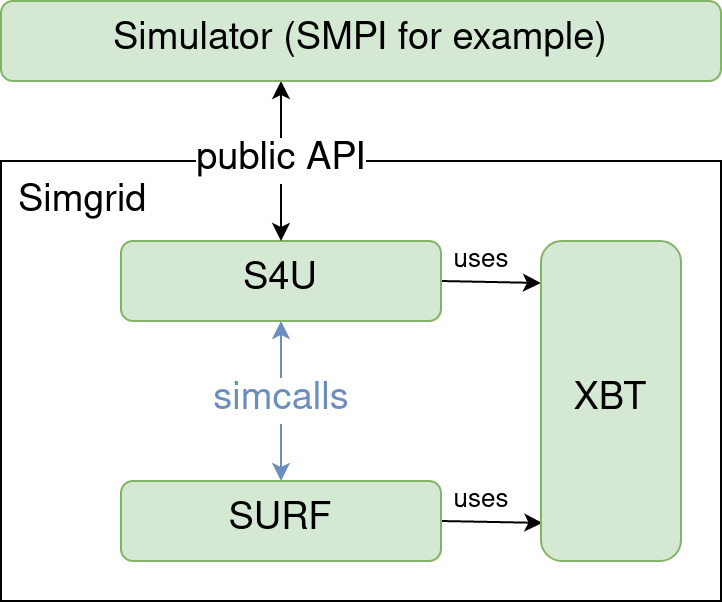
\includegraphics[width=0.5\textwidth]{3_related_work_simu/simgrid_arch.jpg}
    \caption{SimGrid's architecture}
    \label{fig:3_related_work_simu:SimGrid_arch}
\end{figure}

Internally, SimGrid is made of three layers (as seen in
Figure~\ref{fig:3_related_work_simu:SimGrid_arch}): at the lowest level, XBT
(eXtended Bundle of Tools) is a collection of optimized C function to manipulate
data structures, timers and other utilities. On top of it, the simulation kernel
(called SURF) manages the virtual time and resources: it is in this layer that
the duration of Activities (network, IO or compute) is computed in order to
progress the virtual time and schedule the next piece of user code to be
executed. The highest level is called S4U (Simgrid For You) and it implements
the ``public'' API that is exposed to users. It provides abstractions for
low-level concepts using C++ classes, representing the various resources that
user code can interact with: Hosts represent simulated pieces of hardware (like
a full machine, or a part of a machine) and Links represent any cable (usually
network cables) that connects Hosts. Additionally, S4U provides classes to
better abstract user code and communication, namely Actors and Mailboxes. Actors
represent any piece of code that is to be scheduled asynchronously from other
Actors' code, in other terms it will often model a process in the simulated
world (or some hardware's logic that runs independently of other hardware).
Actors need to be instantiated on a specific Host in the simulated platform in
order for SURF to know at which speed computation phases need to be executed.
Mailboxes on the other hand, are a mechanism that allows Actors to communicate:
traditionally, in SimGrid, data transfers will occur when two Actors issue a
``send'' and a ``receive'' call to the same Mailbox (which are identified by a
unique name). By default, Mailboxes are not linked to a specific Host (they are
not ``located'' anywhere on the simulated platform), which means that the Links
used in a communication can only be decided when both the sender and the
receiver have issued their call (\inline{put} to send or \inline{get} to
receive) to the Mailbox. Indeed, this is only at this instant that SURF will be
able to determine which Hosts are communicating. This means that Mailboxes
effectively work as ``rendezvous'' points, although it is possible to set a
specific Actor as a ``permanent receiver'' for a Mailbox, which allows the
transfer to start at soon as a ``send'' is issued on the Mailbox (before any
``receive''). This mechanic is depicted in
Figure~\ref{fig:3_related_work_simu:SimGrid_mailboxes}, and it will be used
extensively in our simulator, which will be described in more detail in
Chapter~\ref{chap:low_level}.

\begin{figure}[!ht]
    \centering
    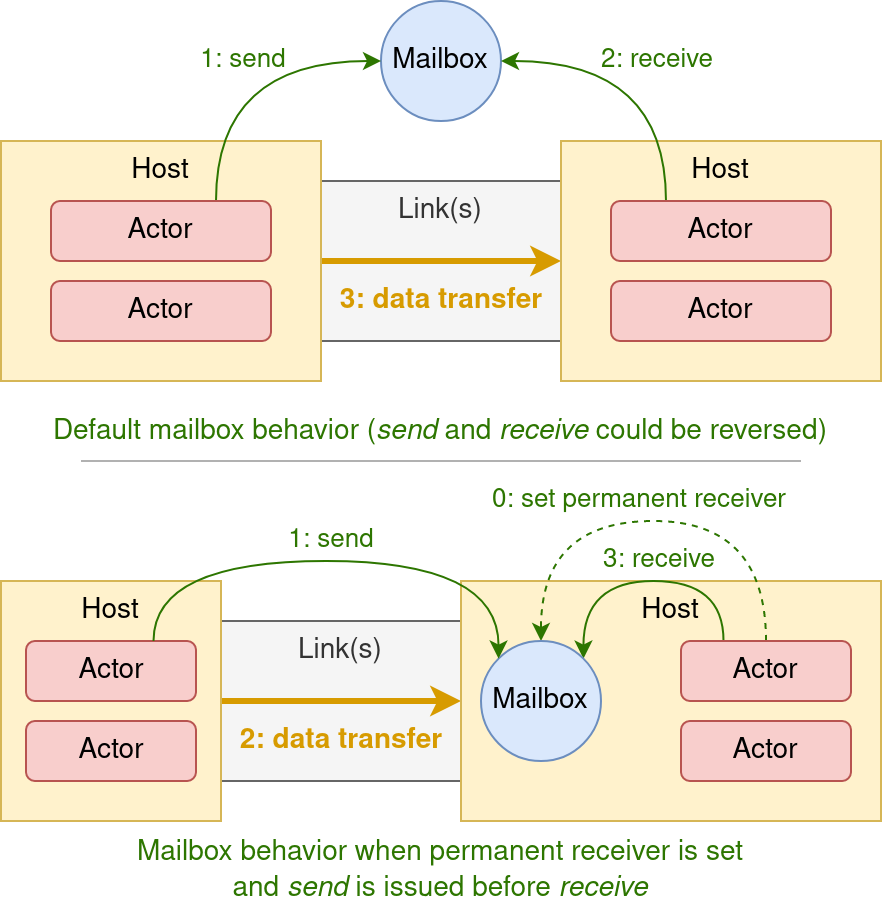
\includegraphics[width=0.7\textwidth]{3_related_work_simu/simgrid_mailboxes.png}
    \caption{SimGrid's mailbox system}
    \label{fig:3_related_work_simu:SimGrid_mailboxes}
\end{figure}

SimGrid uses cooperative actors, and it is architectured in a way that is heavily
inspired by operating systems: indeed, the user-space interface (S4U)
communicates with the simulation kernel (SURF) using a mechanism called
``simcalls'', which are very similar to syscalls on Linux. A simcall is issued
by an Actor each time it needs to perform an operation that might impact the
simulated time (any computation, communication or IO). Effectively simcalls are
a way for Actors to ask SURF to perform the desired operation and wake them up
again either at the same date in the simulated world (in case of asynchronous
operations), or whenever the operation is completed (in the case of synchronous
operation), so each time an Actor performs a simcall it will yield to the kernel
and trigger a new scheduling round. This only happens when Actors perform
simcall, as SimGrid simulations are cooperative, therefore it is the
responsibility of Actors to yield (either using a simcall or by calling a
dedicated primitive to do it explicitly).

\subsection{Usage}

While SimGrid is programmed with C++ 17, it offers bindings in C++ and Python. A
Java interface also used to exist for the old MSG user API, but it has not been
maintained when MSG was deprecated in favor of the S4U interface. During this
thesis we use exclusively the C++ S4U interface. An example of a toy simulation
using this interface is shown on
Figure~\ref{fig:3_related_work_simu:SimGrid_pingpong}.

\begin{figure}[!ht]
    \lstinputlisting[basicstyle=\ttfamily\scriptsize,frame=bt,language=C++]{3_related_work_simu/simgrid_pingpong.cpp}
    \caption{Simplistic ping-pong with SimGrid's S4U interface}
    \label{fig:3_related_work_simu:SimGrid_pingpong}
\end{figure}

In this example, which implements a ping-pong with exponential message sizes,
first our two Actor types are defined: \inline{initiator} to start the
``pings'', and \inline{target} which will receive them and send ``pongs'' back.
Their behaviors are simply a function, because that is sufficient for this
simple example, but SimGrid supports making Actors from anything that is
callable in C++, including objects (by overloading the \inline{()} operator,
which we will use extensively in this thesis). The initiator Actor simply sends
``pings'' of increasing size, attaching a sequence number to each message
(\inline{iteration}), and waits for ``pongs'', checking that the ``pong''
sequence number is the same that was sent. The target ``daemonizes'' itself,
which means that the simulation will end (and this Actor will be killed
automatically) when all the other Actors are done executing their logic (which
means that the end of the initiator will trigger the end of the simulation in
this case). While this example is very simple, it already shows a few
interesting things about SimGrid: First, we can see how the XBT layer can be
used for several utility purposes, like an assertion API and a logging system.
This logging system is very complete, and is used through C-style macros that
mimic the \inline{printf} API. Even though that is not showcased in this
simplistic example, it supports a tree-like structure of categories and
subcategories, which enables fine-tuning on the command line which level of log
to display for each category. In the Actors' code we can see the S4U API being
used to interact with the Mailbox system in order to send and receive messages.
As most resources in SimGrid, Mailboxes follow the RAII paradigm (Resource
Acquisition Is Initialization), therefore we do not have to instantiate the
Mailbox ourselves, we simply ask SimGrid to give us a Mailbox with that name,
and internally S4U will either return it to us if it already exists or create it
if it does not. This means that in our example, we do not know if the two
mailboxes are going to be created from the \inline{s4u::Mailbox::by_name} calls
from initiator or the target (since all this code happens at $t = 0$ in the
simulated world), but it does not matter since the result is going to be
identical. It is worth noting that even if we managed to cause a potential race
condition (because of two Actors executing code at the same simulated time), it
is easier to debug in simulation compared to a real-world execution, because
even though the order of operation happening at the same simulated time is
random from a user perspective, it is deterministic, to ensure the
reproducibility of SimGrid's simulation. Finally, the \inline{main} function
sets up the simulation, declaring our Actors, and loading the platform and
deployment from XML files before starting the simulation Engine. The output of
this toy simulation is displayed on
Figure~\ref{fig:3_related_work_simu:Pingpong_output}. We can see that even
though SimGrid provides methods to get the simulated time, we did not need to
use them, as the logging system from XBT already prints the current Actor,
simulated time, category and log level on each line.

\begin{figure}[!t]
    \lstinputlisting[basicstyle=\ttfamily\scriptsize,frame=bt]{3_related_work_simu/pingpong_output.txt}
    \caption{Ping-pong's output}
    \label{fig:3_related_work_simu:Pingpong_output}
\end{figure}

\subsection{Performance and isolation concerns}

Despite being used to build single-threaded simulators, SimGrid has demonstrated
a very good scalability thanks in particular to its platform
representation~\cite{Bobelin2012} and the optimization of its sequential
Discrete Event Simulation (DES) kernel~\cite{Degomme2017a}. This is because a
DES requires many synchronizations, since there is a central value of the
current simulated time that is shared by all Actors in the system, making
parallelism very difficult. Some simulation frameworks try to use several
threads regardless, or to work on top of MPI to distribute work on several
machines (which is the case of the SST for example). The approach used varies,
for example ROSS~\cite{Carothers2002} uses an optimistic scheduler to reduce the
number of synchronizations required to the minimum, but this means that
backtracking might be required when an inconsistency is detected. This makes
simulators harder to write (since they need to implement rollback mechanisms),
and it also limits the speedup that can be obtained from parallelization. Having
a sequential DES also makes writing a simulator significantly easier: race
conditions can still happen due to the asynchronous nature of the simulation,
but most data structures can be used safely with no synchronization since Actors
are executed one at a time, and therefore cannot access a piece of data at the
same wallclock time.

The biggest issue that arises from having a single-threaded simulator is that
all Actors share the same memory space. To work around this issue, and have a
dedicated stack for each Actor, SimGrid allocates a tunable amount of memory to
each Actor's stack, and when switching context from one Actor to the other it
provides different mechanisms: either using a full thread for each Actor, but
with only one running at any given time (which is a very portable solution but
very slow), \inline{ucontext} from the System V API (which are faster but
available only on Linux and FreeBSD), boost contexts (which are also reasonably
fast but add a dependency), and finally ``raw'' contexts, which are implemented
by SimGrid directly in x86 and amd64 assembly code. This last solution is
extremely fast, as it requires only a few CPU cycles to switch contexts. Its
only two downsides are that it is not portable to other CPU architectures, and
that this way of moving registers manually can make debugging much harder (in
tools like GDB for example). For this reason, in this thesis we use ``thread''
context when debugging is needed (as it is very compatible with standard tools),
and ``raw'' contexts when making full scale experiments.

To describe the simulated platform, on which Actors will be instantiated,
SimGrid provides several interfaces. The most common one is through a static XML
file, which is a list of Hosts, Links, and Routes to describe which Links are
used to communicate between two Hosts. Additionally, some extra tags allow a
more concise description of the platform, such as Router or Cluster to describe
common topologies, but they are simply syntactic sugar and do not add any
feature. This simulated hardware can also be grouped in NetZones that help
describing heterogeneous platforms. Because a static platform can be very
verbose (and the parsing of XML can have an important negative impact on
performance for large platforms), SimGrid also exposes a programmatic API, which
helps describe regular topologies with loops for example. At the beginning of
this thesis this API used to be simplistic and required users to describe their
platform in Lua, but it has since been deprecated in favor of a C++ API that is
much more powerful. Although we started by using SimGrid with the XML
description, we switched to the C++ API when it became available, therefore all
our experiments will use this interface.

Finally, SimGrid offers a system of Plugins, which allows users to listen to
events and extend the features natively offered by the framework. The most
popular are the Energy and Filesystem plugins, which allow users to respectively
estimate the power consumption of hardware, and model a complete Filesystem on
top of the basic Storage features natively offered by SimGrid. We did not use
the plugin system intensively in this thesis.

\section{High-level models}

While some specific parts of MPI have been studied in depth, such as the
matching engine~\cite{Levy2019}, it is very hard to fully model a complete MPI
implementation In HPC, there are two traditional approaches to model high-level
APIs, such as MPI or OpenSHMEM for example. The offline approach requires
obtaining a trace of the communications from a real-world execution, and then
replaying it in simulation, potentially with different parameters, as we
presented earlier. Such studies allow very fast simulation but require users to
be able to obtain a realistic trace in the first place, which can be
problematic. The online approach usually involves re-implementing the whole API
on top of a simulation framework, in order to intercept communication primitives
during the runtime of the application. While this requires a lot of work, it is
the most commonly used, for example by SMPI~\cite{Degomme2017a},
xSim~\cite{Bohm2011} or SST/Macro~\cite{Hendry}, which all provide a complete
MPI implementation in simulation (SMPI even goes as far as implementing several
algorithms for each operation to mimic different real-word implementations of
the MPI standard). Another approach would be to run a real-world API on top of a
simulated low-level network library. While this makes the development of the
simulator easier (since low-level libraries are usually more simplistic than
high-level APIs), it proves very difficult to provide a simulated environment
that is realistic enough to run the high-level API unmodified, which is why this
approach is seldom used. We found an example of it in~\cite{Knight2018}, which
manages to run the GASNet runtime on top of a simulated uGNI implementation
(based on SST), although running more common APIs such as OpenMPI are left as
future work. This last approach will be implemented for OpenMPI and OpenSHMEM
over a simulated Portals implementation (using SimGrid) in this thesis, using
different technical solutions than~\cite{Knight2018} to overcome the challenges
that arise in the process (and which are described in detail in
Chapter~\ref{chap:high_level}).

\section{Multi-level modeling}

Because the performance / accuracy tradeoff of simulators is their biggest
limitation, some studies have tried to make it more dynamic. For example,
Behavioral Emulation~\cite{Ramaswamy2018} tries to add this type of feature to
the SST, by allowing users to write models of various granularity for each type
of hardware. While this is an interesting project, it is very costly to use in
terms of development time, because it is the responsibility of users to write
each model at each granularity that they wish to study. Some simulators also
feature options to make their low-level faster at the cost of some accuracy, for
example by ignoring very short events, but from our experiments this type of
configuration usually has a limited impact on performance and accuracy, as the
underlying model is mostly the same in the end.
